%%% Nordic PGDAY 2015
%%%
%%% A 50 minutes advanced SQL session. You had no idea you could do that in
%%% SQL, and you didn't expect what I'm showing here to be that much easier
%%% in SQL than in whatever your current favorite programming language is.
%%%
%%%  As a developer with solid roots and well into 2014, are ready to
%%% reconsider your SQL usage?

\documentclass{beamer}

\usepackage{minted}
%% \usemintedstyle{emacs}
\usepackage{beamerthemesplit}
\usepackage[utf8]{inputenc}
%% \usetheme{AnnArbor}
\usetheme{Boadilla}
%% \usetheme{Pittsburgh}
%% \usecolortheme{beaver}
%% \beamertemplatetransparentcovered

\title{PostgreSQL for Developers}
\subtitle{Nordic pgDay 2015, Copenhagen}
\author{Dimitri Fontaine \texttt{dimitri@2ndQuadrant.fr}}
\date{March 11, 2015}
\logo{
\includegraphics[height=0.4cm]{2ndQuadrant-cross.png}}

\begin{document}

\frame{\titlepage}

\section{Introduction}

\begin{frame}[fragile]
  \frametitle{Dimitri Fontaine}

  \begin{center}
    \textbf{2ndQuadrant France}
    \linebreak
    PostgreSQL Major Contributor
  \end{center}
  \vfill

\begin{columns}[c]
\column{.75\textwidth} 

  \begin{itemize}
   \item \texttt{pgloader}
   \item \texttt{prefix}, \texttt{skytools}, \texttt{debian}, …
   \item \texttt{\textbf{CREATE EXTENSION}}
   \item \texttt{\textbf{CREATE EVENT TRIGGER}}
  \end{itemize}  

\column{.25\textwidth}
\begin{center}
  
\includegraphics[height=5em]{bulle-blue-icon.png}
\end{center}
\end{columns}
\end{frame}

\begin{frame}[fragile]
  \frametitle{Tools and development languages}

  \center{You're already using plenty of tools and languages already I'm
    sure, let's look at a typical web developer environment}

\begin{columns}[c]
\column{.3\textwidth} 

  \begin{itemize}
   \item HTML
   \item Javascript
   \item \textit{JQuery}
   \item \alert{SQL}
  \end{itemize}  

\column{.7\textwidth}
  \begin{center}
    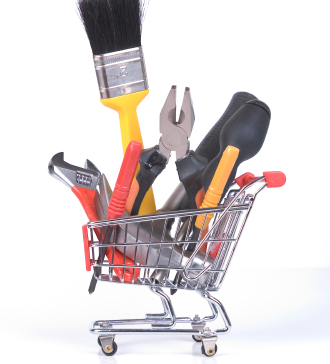
\includegraphics[height=13em]{skill-set.jpg}
  \end{center}
\end{columns}
\end{frame}

\section{Projet}

\frame{
  \frametitle{A simple project}

\begin{center}
  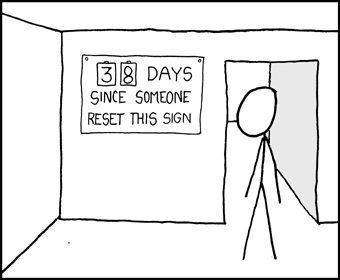
\includegraphics[height=2.3in]{reset.png}
\end{center}    
}

\begin{frame}[fragile]
  \frametitle{Project definition and scope}

  Let's try and solve so,ething simple to get started:

  \begin{itemize}
    \item Managing a counter that can recycle
    \item Adding new measures in a time based fashion
    \item Do monthly reports to allow for invoicing
    \item Analyze the counter behavior
  \end{itemize}
\end{frame}

\begin{frame}[fragile]
  \frametitle{SQL: we start with DDLs}

  \center{\textbf{\textit{Joe Celko}}: \texttt{80\%} of the job is to define
    the schema}
  \vfill

\begin{example}[DDL]
\begin{verbatim}
create table mesures(date timestamptz primary key,
                     mesure integer);

dim=# \d mesures
\d mesures
            Table "public.mesures"
 Column |           Type           | Modifiers 
--------+--------------------------+-----------
 date   | timestamp with time zone | not null
 mesure | integer                  | 
Indexes:
    "mesures_pkey" PRIMARY KEY, btree (date)
\end{verbatim}
\end{example}
\end{frame}

\begin{frame}[fragile]
  \frametitle{We take a very simple model for the presentation}

\begin{minted}{postgresql}
create table measures(tick int, nb int);

insert into measures
     values (1, 0), (2, 10), (3, 20), (4, 30), (5, 40),
            (6, 0), (7, 20), (8, 30), (9, 60);
\end{minted}
\end{frame}

\begin{frame}[fragile]
  \frametitle{Testing data}

  Let's take some measures as if they came out of our counter, starting at
  0, and with a \textit{reset} in there. In that example, the global usage
  measured is \texttt{40 + 60 = 100}.

\begin{minted}{postgresql}
select * from measures;
 tick | nb 
------+----
    1 |  0
    2 | 10
    3 | 20
    4 | 30
    5 | 40
    6 |  0
    7 | 20
    8 | 30
    9 | 60
(9 rows)
\end{minted}
\end{frame}

\begin{frame}[fragile]
  \frametitle{Aside: PostgreSQL knows about arrays}

\begin{minted}{postgresql}
select array_agg(nb) from measures;
         array_agg          
----------------------------
 {0,10,20,30,40,0,20,30,60}
(1 row)
\end{minted}
\end{frame}

\begin{frame}[fragile]
  \frametitle{Finding the last counter value before \textit{reset}}

\begin{columns}
\column{.65\textwidth}
\center{\textit{Write some \alert{SQL} here}}
\column{.35\textwidth}
\begin{minted}{postgresql}
 tick | nb | max 
------+----+-----
    1 |  0 |    
    2 | 10 |    
    3 | 20 |    
    4 | 30 |    
    5 | 40 |  40
    6 |  0 |    
    7 | 20 |    
    8 | 30 |    
    9 | 60 |  60
(9 rows)
\end{minted}
\end{columns}
\end{frame}

\begin{frame}[fragile]
  \frametitle{Window Functions: \texttt{lead() over()}}

\begin{columns}
\column{.65\textwidth}
\begin{minted}{postgresql}
  select tick,
         nb,
         lead(nb) over (order by tick)
    from measures;
\end{minted}

\column{.35\textwidth}
\begin{minted}{postgresql}
 tick | nb | lead 
------+----+------
    1 |  0 |   10
    2 | 10 |   20
    3 | 20 |   30
    4 | 30 |   40
    5 | 40 |    0
    6 |  0 |   20
    7 | 20 |   30
    8 | 30 |   60
    9 | 60 |     
(9 rows)
\end{minted}
\end{columns}
\end{frame}

\begin{frame}[fragile]
  \frametitle{Window Functions and \texttt{CASE}}

\begin{columns}
\column{.65\textwidth}
\begin{minted}{postgresql}
  select tick, nb,
         case when lead(nb) over w < nb
              then nb

              when lead(nb) over w is null
              then nb

              else null
          end as max
    from measures
  window w as (order by tick);
\end{minted}
\column{.35\textwidth}
\begin{minted}{postgresql}
 tick | nb | max 
------+----+-----
    1 |  0 |    
    2 | 10 |    
    3 | 20 |    
    4 | 30 |    
    5 | 40 |  40
    6 |  0 |    
    7 | 20 |    
    8 | 30 |    
    9 | 60 |  60
(9 rows)
\end{minted}
\end{columns}
\end{frame}

\begin{frame}[fragile]
  \frametitle{Window Functions and \texttt{WHERE} clause}

\begin{minted}{postgresql}
with t(tick, nb, max) as (
  select tick, nb,
         case when lead(nb) over w < nb then nb
              when lead(nb) over w is null then nb
              else null
          end as max
    from measures
  window w as (order by tick)
)
select tick, nb, max from t where max is not null;
 tick | nb | max 
------+----+-----
    5 | 40 |  40
    9 | 60 |  60
(2 rows)
\end{minted}
\end{frame}

\begin{frame}[fragile]
  \frametitle{Common Table Expressions to complement \texttt{WITH}}

\begin{minted}{postgresql}
with t(tops) as (
  select case when lead(nb) over w < nb then nb
              when lead(nb) over w is null then nb
              else null
          end as max
    from measures
  window w as (order by tick)
)
select sum(tops) from t;
 sum 
-----
 100
(1 row)
\end{minted}
\end{frame}

\frame{
  \frametitle{Getting usage from the counter: done. SQL. 9 lines.}

  \begin{center}
    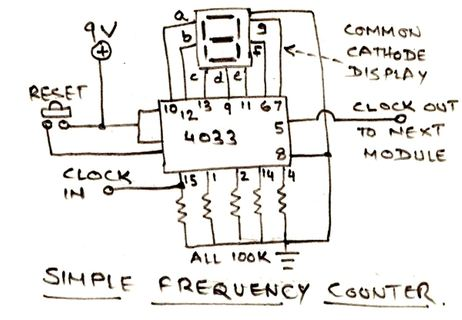
\includegraphics[height=2.3in]{reset-circuit-thumbnail.jpg}
  \end{center}
}

\begin{frame}[fragile]
  \frametitle{Let's test with more than one cycle}

\begin{minted}{postgresql}
insert into measures
     values (10, 0), (11, 10), (12, 30), (13, 35), (14, 45),
            (15, 25), (16, 50), (17, 100), (18, 110);
\end{minted}
\end{frame}

\begin{frame}[fragile]
  \frametitle{Visualizing the cycles}

\begin{minted}{postgresql}
with t(tick, nb, max) as (
  select tick, nb,
         case when lead(nb) over w < nb then nb
              when lead(nb) over w is null then nb
              else null
          end as max
    from measures
  window w as (order by tick)
)
select tick, nb, max from t where max is not null;
 tick | nb  | max 
------+-----+-----
    5 |  40 |  40
    9 |  60 |  60
   14 |  45 |  45
   18 | 110 | 110
(4 rows)
\end{minted}
\end{frame}


\begin{frame}[fragile]
  \frametitle{Resource usage, with several cycles}

\begin{minted}{postgresql}
with t(tops) as (
  select case when lead(nb) over w < nb then nb
              when lead(nb) over w is null then nb
              else null
          end as max
    from measures
  window w as (order by tick)
)
select sum(tops) from t;
 sum 
-----
 255
(1 row)
\end{minted}
\end{frame}

\begin{frame}[fragile]
  \frametitle{Limit measure taken into account}

  \begin{center}
    
\includegraphics[height=2.3in]{calendar.png}
  \end{center}
\end{frame}

\begin{frame}[fragile]
  \frametitle{Limit measures period (time range)}

\begin{columns}
\column{.65\textwidth}
\begin{minted}{postgresql}
select tick, nb
  from measures
 where tick >= 4 and tick < 14;
\end{minted}

\column{.35\textwidth}
\begin{minted}{postgresql}
 tick | nb 
------+----
    4 | 30
    5 | 40
    6 |  0
    7 | 20
    8 | 30
    9 | 60
   10 |  0
   11 | 10
   12 | 30
   13 | 35
\end{minted}
\end{columns}
\end{frame}

\begin{frame}[fragile]
  \frametitle{Limit measures period using \texttt{first\_value}}

\begin{columns}
\column{.65\textwidth}
\begin{minted}{postgresql}
  select nb,
     first_value(nb) over w as first,
     case when lead(nb) over w < nb
          then nb

          when lead(nb) over w is null
          then nb

          else null
      end as max
    from measures
   where tick >= 4 and tick < 14
  window w as (order by tick);
\end{minted}

\column{.35\textwidth}
\begin{minted}{postgresql}
 nb | first | max 
----+-------+-----
 30 |    30 |    
 40 |    30 |  40
  0 |    30 |    
 20 |    30 |    
 30 |    30 |    
 60 |    30 |  60
  0 |    30 |    
 10 |    30 |    
 30 |    30 |    
 35 |    30 |  35
(10 rows)
\end{minted}
\end{columns}
\end{frame}

\begin{frame}[fragile]
  \frametitle{Resource usage in a given period}

\begin{minted}{postgresql}
with t as (
  select tick,
         first_value(nb) over w as first,
         case when lead(nb) over w < nb then nb
              when lead(nb) over w is null then nb
              else null
          end as max
    from measures
   where tick >= 4 and tick < 14
  window w as (order by tick)
)
select sum(max) - min(first) as sum from t;
 sum 
-----
 105
(1 row)
\end{minted}
\end{frame}

\begin{frame}[fragile]
  \frametitle{Counter behavior: \textit{reset}}

  \begin{center}
    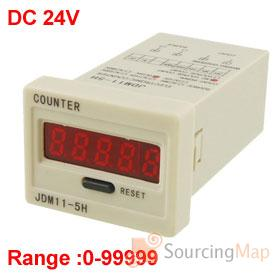
\includegraphics[height=2.3in]{reset-elect.jpg}
  \end{center}
  
\end{frame}

\begin{frame}[fragile]
  \frametitle{Partitionning on the \textit{reset}}

\begin{minted}{postgresql}
with tops as (
  select tick, nb,
         case when lead(nb) over w < nb then nb
              when lead(nb) over w is null then nb
             else null
         end as max
    from measures
  window w as (order by tick)
)
  select tick, nb, max,
         (select tick
            from tops t2
           where t2.tick >= t1.tick and max is not null
        order by t2.tick
           limit 1) as p
    from tops t1;
\end{minted}
\end{frame}

\begin{frame}[fragile]
  \frametitle{Partitioning on \textit{reset}}

\begin{columns}
\column{.5\textwidth}
\begin{minted}{postgresql}
 tick | nb  | max | p  
------+-----+-----+----
    1 |   0 |     |  5
    2 |  10 |     |  5
    3 |  20 |     |  5
    4 |  30 |     |  5
    5 |  40 |  40 |  5
    6 |   0 |     |  9
    7 |  20 |     |  9
    8 |  30 |     |  9
    9 |  60 |  60 |  9
\end{minted}

\column{.5\textwidth}
\begin{minted}{postgresql}
 tick | nb  | max | p  
------+-----+-----+----
   10 |   0 |     | 14
   11 |  10 |     | 14
   12 |  30 |     | 14
   13 |  35 |     | 14
   14 |  45 |  45 | 14
   15 |  25 |     | 18
   16 |  50 |     | 18
   17 | 100 |     | 18
   18 | 110 | 110 | 18
\end{minted}
\end{columns}
\end{frame}

\begin{frame}[fragile]
  \frametitle{Time range partitioning with \texttt{PARTITION BY}}

\begin{columns}
\column{.65\textwidth}
\begin{minted}{postgresql}
with tops as ( <case lead() over()> ),
     parts as ( <self join limit 1> ),
     ranges as (
  select
      first_value(tick) over w as start,
      last_value(tick) over w as end,
      max(max) over w
    from parts
  window w as (PARTITION BY p
               order by tick)
)
select * from ranges
 where max is not null;
\end{minted}

\column{.35\textwidth}
\begin{minted}{postgresql}
 start | end | max 
-------+-----+-----
     1 |   5 |  40
     6 |   9 |  60
    10 |  14 |  45
    15 |  18 | 110
(4 rows)
\end{minted}
\end{columns}
\end{frame}

\begin{frame}[fragile]
  \frametitle{PostgreSQL knows about ranges: \texttt{in4range()}}

\begin{columns}
\column{.65\textwidth}
\begin{minted}{postgresql}
with tops as ( <case lead() over()> ),
     parts as ( <self join limit 1> ),
     ranges as (
  select int4range(
           first_value(tick) over w,
           last_value(tick) over w,
           '[]') as range,
         max(max) over w as compteur
    from parts
  window w as (partition by p
               order by tick)
)
select range, compteur
  from ranges
 where compteur is not null;
\end{minted}
\column{.35\textwidth}
\begin{minted}{postgresql}
  range  | compteur 
---------+----------
 [1,6)   |       40
 [6,10)  |       60
 [10,15) |       45
 [15,19) |      110
(4 rows)
\end{minted}
\end{columns}
\end{frame}

\begin{frame}[fragile]
  \frametitle{Usage by range using \texttt{@>}}

\begin{columns}
\column{.65\textwidth}
\begin{minted}{postgresql}
with tops as ( <case lead() over()> ),
     parts as ( <self join limit 1> ),
     ranges as ( <int4range()
                  over (partition by
                        order by)> )
select range, compteur
  from ranges
 where compteur is not null
       and range @> 11;
\end{minted}

\column{.35\textwidth}
\begin{minted}{postgresql}
  range  | compteur 
---------+----------
 [10,15) |       45
(1 row)
\end{minted}
\end{columns}
\end{frame}

\section{Extra}

\begin{frame}[fragile]
  \frametitle{Extensions and data types}

\begin{center}
  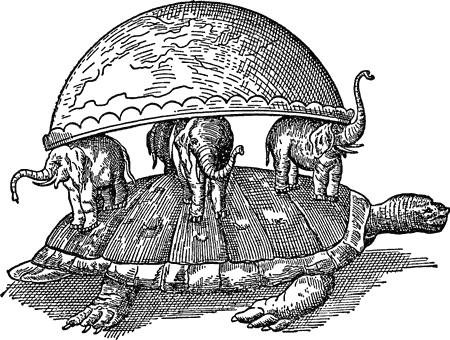
\includegraphics[height=18em]{extensions.png}
\end{center}
\end{frame}

\begin{frame}[fragile]
  \frametitle{Some extensions example}

  \center{46 Contribs, Community extensions, Private ones...}
  \vfill

\begin{columns}[c]

\column{.18\textwidth}
  \begin{itemize}
   \item \alert{hll}
   \item cube
   \item \alert{ltree}
   \item citext
   \item \alert{hstore}
  \end{itemize}

\column{.25\textwidth}
  \begin{itemize}
   \item \alert{earthdistance}
   \item pgq
   \item \alert{pg\_trgm}
   \item wildspeed
   \item \alert{plproxy}
  \end{itemize}

\column{.21\textwidth} 
  \begin{itemize}
   \item PostGIS
   \item \alert{ip4r}
   \item \alert{intarray}
   \item \alert{prefix}
   \item pgfincore
  \end{itemize}

\column{.4\textwidth}
  \begin{itemize}
   \item pgcrypto
   \item pg\_stattuple
   \item pg\_buffercache
   \item pg\_stat\_statements
   \item \alert{pgfincore}
  \end{itemize}

\end{columns}
\end{frame}

\section{IP Ranges with ip4r}

\begin{frame}[fragile]
  \frametitle{IP Ranges, \texttt{ip4r}}

\begin{center}
  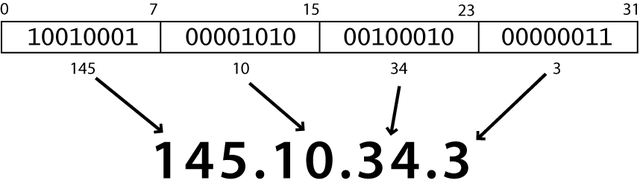
\includegraphics[height=6em]{ip-address.png}
\end{center}
\end{frame}

\begin{frame}[fragile]
  \frametitle{IP Ranges, \texttt{ip4r}}

\begin{columns}
\column{.7\textwidth}
\begin{minted}{postgresql}
table geolite.blocks limit 10;
        iprange        | locid 
-----------------------+-------
 1.0.0.0/24            |    17
 1.0.1.0-1.0.3.255     |    49
 1.0.4.0/23            | 14409
 1.0.6.0/23            |    17
 1.0.8.0/21            |    49
 1.0.16.0/20           | 14614
 1.0.32.0/19           | 47667
 1.0.64.0/18           |   111
 1.0.128.0-1.0.147.255 |   209
 1.0.148.0/24          | 22537
(10 rows)
\end{minted}
\end{columns}
\end{frame}

\begin{frame}[fragile]
  \frametitle{IP Ranges, \texttt{ip4r}, Geolocation}

  \center{PostgreSQL allows using SQL and JOINs to match IP4R with geolocation.}
  \vfill

\begin{columns}
\column{.45\textwidth}
\begin{minted}{postgresql}
 select *
   from geolite.blocks
   join geolite.location
        using(locid)
  where iprange
            >>=
        '74.125.195.147';
\end{minted}
\column{.55\textwidth}
\begin{center}
  
\includegraphics[height=9em]{geolocation-clic.png}
\end{center}
\end{columns}
\end{frame}

\begin{frame}[fragile]
  \frametitle{IP Ranges, \texttt{ip4r}, Geolocation}

  \center{PostgreSQL allows using SQL and JOINs to match IP4R with geolocation.}
  \vfill

\begin{columns}
\column{.45\textwidth}
\begin{minted}{postgresql}
 select *
   from geolite.blocks
   join geolite.location
        using(locid)
  where iprange
            >>=
        '74.125.195.147';
\end{minted}
\column{.55\textwidth}
\begin{minted}{postgresql}
-[ RECORD 1 ]----------------------------
locid      | 2703
iprange    | 74.125.189.24-74.125.255.255
country    | US
region     | CA
city       | Mountain View
postalcode | 94043
location   | (-122.0574,37.4192)
metrocode  | 807
areacode   | 650

Time: 1.335 ms
\end{minted}
\end{columns}
\end{frame}

\section{Earth Distance}

\begin{frame}[fragile]
  \frametitle{Earth Distance}

\begin{center}
  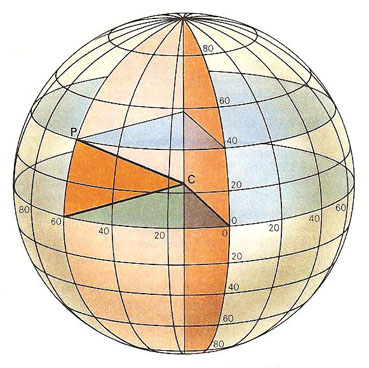
\includegraphics[height=15em]{latitude_and_longitude.jpg}
\end{center}
\end{frame}

\begin{frame}[fragile]
  \frametitle{How Far is The Nearest Pub}

  \center{The \texttt{point} datatype is in-core}
  \vfill

\begin{columns}[c]
\column{.45\textwidth} 

\begin{minted}{postgresql}
#  CREATE TABLE pubnames
   (
     id   bigint,
     pos  POINT,
     name text
   );
\end{minted}  

\column{.55\textwidth}
\begin{center}
  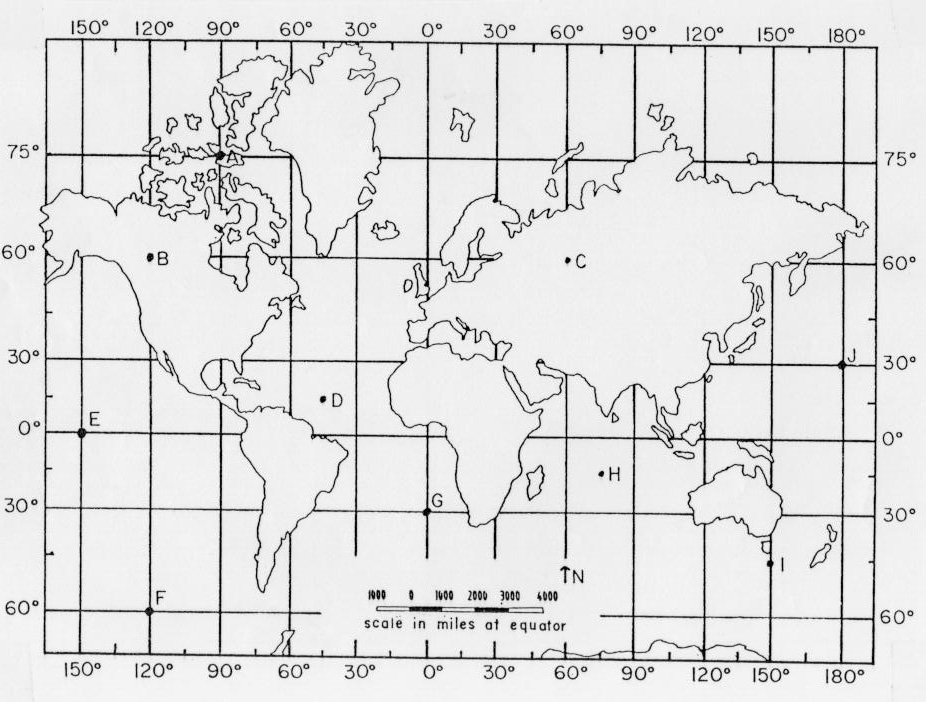
\includegraphics[height=9em]{ltlng.jpg}
\end{center}
\end{columns}
\end{frame}

\begin{frame}[fragile]
  \frametitle{How Far is The Nearest Pub}

\begin{minted}{postgresql}
  select name, pos
    from pubnames
order by pos <-> point(-6.25,53.346)
    limit 3;

          Pub Name          |           pos           
----------------------------+-------------------------
 Ned's                      | (-6.2519967,53.3458267)
 Sub Lounge                 | (-6.2542332,53.3469085)
 O'Neill's of Pearse Street | (-6.2524389,53.3448589)
(3 rows)

Time: 18.679 ms
\end{minted}  
\end{frame}

\begin{frame}[fragile]
  \frametitle{How Far is The Nearest Pub}

\begin{center}
\begin{minted}{postgresql}
CREATE INDEX on pubnames USING GIST(pos);
\end{minted}  
\end{center}
\vfill

\begin{columns}
\column{.65\textwidth}
\begin{minted}{postgresql}
  select name,
         pos
    from pubnames
order by pos <-> point(-0.12,51)
   limit 3;
\end{minted}  

\column{.35\textwidth}
\begin{minted}{postgresql}
  name  |      pos           
--------+--------------
 Ned's  | (-6.25,53.34)
 Sub Lo | (-6.25,53.34)
 O'Neil | (-6.25,53.34)
(3 rows)

Time: 0.849 ms
\end{minted}  
\end{columns}
\end{frame}

\begin{frame}[fragile]
  \frametitle{How Far is The Nearest Pub, in Miles please.}

\begin{minted}{postgresql}
create extension cube;
create extension earthdistance;
\end{minted}  
\vfill

\begin{columns}
\column{.65\textwidth}
\begin{minted}{postgresql}
  select name,
   pos <@> point(-6.25,53.34) miles
    from pubnames
order by pos <-> point(-6.25,53.34)
   limit 3;
\end{minted}  
\column{.35\textwidth}
\begin{minted}{postgresql}
  name  | miles 
--------+-------
 Ned's  |  0.06
 Sub Lo |  0.07
 O'Neil |  0.12
(3 rows)

Time: 1.335 ms
\end{minted}  
\end{columns}
\end{frame}

\begin{frame}[fragile]
  \frametitle{Some pubs far away from here...}

\begin{columns}
\column{.65\textwidth}
\begin{minted}{postgresql}
  select c.name as city,
  pos <@> point(-6.25,53.34) as miles
   from pubnames p,
     lateral (select name
                from cities c
            order by c.pos <-> p.pos
               limit 1) c
 order by pos <-> point(-6.25,53.34)
           desc
    limit 5;
\end{minted}  
\column{.35\textwidth}
\begin{minted}{postgresql}
    city    |  miles       
------------+--------
 Canterbury | 399.44
 Canterbury | 378.91
 Canterbury | 392.08
 Canterbury | 397.30
 Canterbury | 379.68
(5 rows)

Time: 636.445 ms
\end{minted}  
\end{columns}
\end{frame}

\begin{frame}[fragile]
  \frametitle{Geolocation: \texttt{ip4r} meets \text{earthdistance}}

\begin{center}
  
\includegraphics[height=12em]{geolocation.png}
\end{center}
\end{frame}

\begin{frame}[fragile]
  \frametitle{Some pubs nearby... some place...}

\begin{columns}
\column{.5\textwidth}
\begin{minted}{postgresql}
with geoloc as
 (
  select location as l
    from location
    join blocks using(locid)
   where iprange
         >>=
         '212.58.251.195'
 )
  select name,
         pos <@> l miles
    from pubnames, geoloc
order by pos <-> l
   limit 10;
\end{minted}  
\column{.5\textwidth}
\begin{minted}{postgresql}
        name        | miles 
--------------------+-------
 Blue Anchor        | 0.299
 Dukes Head         | 0.360
 Blue Ball          | 0.337
 Bell (aka The Rat) | 0.481
 on the Green       | 0.602
 Fox & Hounds       | 0.549
 Chequers           | 0.712
 Sportsman          | 1.377
 Kingswood Arms     | 1.205
 Tattenham Corner   | 2.007
(10 rows)

Time: 3.275 ms
\end{minted}  
\end{columns}
\end{frame}

\section{Conclusion}

\frame{
  \frametitle{Conclusion}

\begin{center}
  You are already using SQL, make the best out of it!
  \vfill

  \begin{center}
    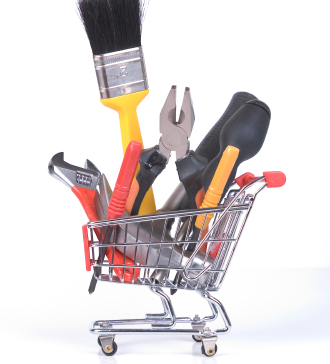
\includegraphics[height=2.1in]{skill-set.jpg}
  \end{center}
\end{center}
}

\end{document}
